\documentclass[a4paper,10pt]{article}
\usepackage[utf8]{inputenc}
\usepackage[colorlinks,plainpages=false]{hyperref}

\setlength\parindent{0pt}
\usepackage[english]{babel}
\usepackage[dvinames]{xcolor}
\usepackage[compact,small]{titlesec}
\usepackage{booktabs}
\usepackage{multirow}
\usepackage{amsfonts,amsmath,amssymb}
\usepackage{marginnote}
\usepackage[top=1.8cm, bottom=1.8cm, outer=1.8cm, inner=1.8cm, heightrounded, marginparwidth=2.5cm, marginparsep=0.5cm]{geometry}
\usepackage{enumitem}
\setlist{noitemsep,parsep=2pt}
\newcommand{\highlight}[1]{\textcolor{kuleuven}{#1}}
\usepackage{pythonhighlight}
\usepackage{cleveref}
\usepackage{graphicx}
\graphicspath{{Pictures/}}
\usepackage{algorithmic}
\usepackage{tabularx}
\usepackage{bm}
\usepackage{subcaption}


\newcommand{\nextyear}{\advance\year by 1 \the\year\advance\year by -1}
\newcommand{\thisyear}{\the\year}
\newcommand{\deadlineGroup}{November 27, \thisyear{} at 16:00 CET}
\newcommand{\deadlineCode}{December 18, \thisyear{} at 16:00 CET}
\newcommand{\deadlineReport}{January 4, \nextyear{} at 16:00 CET}

\newcommand{\ReplaceMe}[1]{{\color{blue}#1}}
\newcommand{\RemoveMe}[1]{{\color{purple}#1}}

\setlength{\parskip}{5pt}

%opening
\title{Artificial Neural Networks: Exercise session 3}
\author{Stijn Staring (r0620003)}

\begin{document}
\fontfamily{ppl}
\selectfont{}

\maketitle


\section{Principal Component Analysis}
Principal component analysis is a method for dimensionality reduction. A principal component analysis uses the eigenvectors of the covariance matrix of the original data as principal components to conduct a linear transformation of the original data to a lower dimension. The eigenvectors that correspond to the largest eigenvalues are considered the most important principal components that determine data appearance the most.

\begin{equation}\label{eq:form1}
	\bm{z} = \bm{E}^T\bm{x}.
\end{equation}

In Eq. \ref{eq:form1}, $ \bm{x} $ is an original data point with dimensions $ \mathbb{R}^p $ and $ \bm{z} $ is the corresponding data point with reduced dimensions $ \mathbb{R}^q $. $ \bm{E}^T $ is the used transformation matrix with dimensions $ q \times p $ and with the $ q $ largest eigenvectors of the covariance matrix as rows. The new dimensions of the data point equals the amount of chosen eigenvectors that span the subspace. If all eigenvalues are distinct, $ \bm{E} $ is orthogonal and the original data point can be retrieved by multiplying Eq. \ref{eq:form1} by $ \bm{E} $ because of the orthogonality property: $ \bm{E}\cdot \bm{E}^{T} = \bm{I} $.\\

The first task performed is the comparison of the dimensionality reduction of random data in comparison to highly correlated data. It is found that there are less eigenvectors needed for the highly correlated data when the same RMSE is considered. The second task is to perform PCA on handwritten images of the digit 3 taken from the US Postal Service database. In this database every image consists out of $ 16 \times 16 $ pixels which is represented by an array of 256 floating numbers. The database consists out of a total of 500 images of the digit 3. When the mean array is calculated, also the mean digit 3 is obtained which is displayed in Figure \ref{fig:mean_three}. The covariance matrix is calculated for the data set and the eigenvalues derived are shown by Figure \ref{fig:50_largest_eigenvalues}. The influence of the amount of eigenvectors is demonstrated in Figure \ref{fig:increasing_eigenvectors}. When only one eigenvector is used, the reduced images are very similar. This means that the eigenvector with the largest eigenvalue focusses on the intrinsic shape of a 3. This means in what distinguishes a 3 from another number e.g. a 5. when more eigenvectors are used and the dimensionality of the spanned subspace increases, different variations of the digit 3 becomes clear. 

\begin{figure}[hb]
	\centering
	\begin{subfigure}[b]{0.49\textwidth}
		\centering
		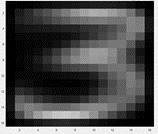
\includegraphics[width=0.55\linewidth]{mean_three.png}
		\caption{Mean image of digit 3}
		\label{fig:mean_three}
	\end{subfigure}
	\begin{subfigure}[b]{0.49\textwidth}
		\centering
		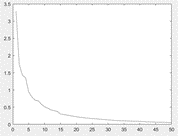
\includegraphics[width=0.6\linewidth]{50_largest_eigenvalues.png}
		\caption{Eigenvalues}
		\label{fig:50_largest_eigenvalues}
	\end{subfigure}
	\begin{subfigure}[b]{1.0\textwidth}
		\centering
		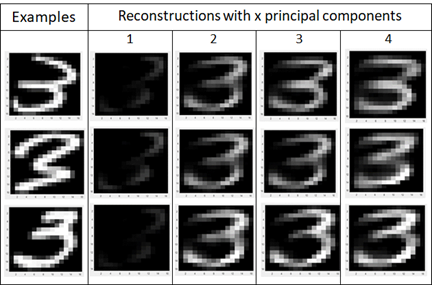
\includegraphics[width=0.4\linewidth]{reconstruction_x_principal_eigenvalues.png}
		\caption{Increasing amount of eigenvectors}
		\label{fig:increasing_eigenvectors}
	\end{subfigure}		
	\caption{Results of applying PCA on the US Postal Service database.}
	\label{fig:Results1}
\end{figure}

In Figure \ref{fig:Results2} the effect of the number of eigenvectors on the RMSE  used in the PCA, is investigated and the distribution of the sizes of the eigenvalues is shown. From Figure \ref{fig:Reconstruction_error1} it is concluded that when more eigenvectors are included, the representation error decreases because the dimensionality is less reduced. When the derivative of the function is assessed, it is found that the function decreases much faster at the beginning than at the end. This means that already by the use of a small amount of eigenvectors to span the subspace with a lower dimensionality, the reconstruction error can be significantly decreased and an already good reconstruction of the original data is possible. Figure \ref{fig:Reconstruction_error2} shows the cumulative sum of eigenvalues used in the PCA with on the x-axis the number of excluded eigenvalues starting from the largest. It is seen that a small amount of eigenvalues have large eigenvalues after which the size decreases rapidly. The plot is similar to Figure \ref{fig:Reconstruction_error1} and it can be concluded that the contribution of an eigenvector in reducing the RMSE corresponds to the size of the eigenvalue. This confirms what was concluded in Figure \ref{fig:Reconstruction_error1}, that already good representations of the digit 3 are possible with a small amount of eigenvectors. When Eq. \ref{eq:form1} is used without a dimensionality reduction, a very small reconstruction error equal to the default floating point precision in Matlab is found. 

\begin{figure}[h]
	\centering
	\begin{subfigure}[c]{0.49\textwidth}
		\centering
		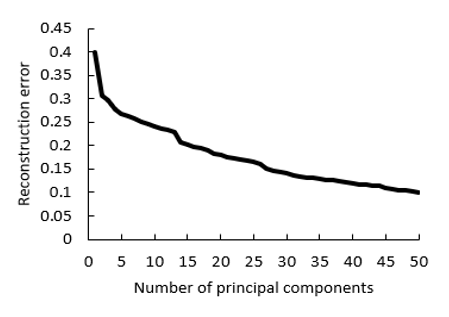
\includegraphics[width=0.85\linewidth]{Reconstruction_error1.png}
		\caption{}
		\label{fig:Reconstruction_error1}
	\end{subfigure}
	\begin{subfigure}[c]{0.49\textwidth}
		\centering
		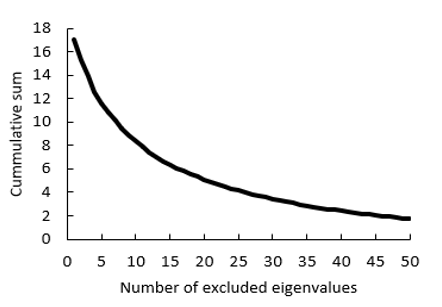
\includegraphics[width=0.8\linewidth]{Reconstruction_error2.png}
		\caption{}
		\label{fig:Reconstruction_error2}
	\end{subfigure}
	\caption{The influence of the amount of eigenvectors used.}
	\label{fig:Results2}
\end{figure}

\section{Stacked Autoencoders}


%\begin{table}
%	\centering
%	\begin{tabular}{@{}clr@{}} \toprule
%		\textbf{Attractor} & \textbf{Point} & \textbf{Stability}\\\midrule
%		Attractor $ 1 $ & $ [1;1] $ & Stable\\
%		Attractor $ 2 $ & $ [-1;-1] $ & Stable\\
%		Attractor $ 3 $ & $ [1;-1] $ & Stable\\
%		Attractor $ 4 $ & $ [-1;1] $ & Stable\\
%		Attractor $ 5 $ & $ [0;0] $ & Unstable\\
%		Attractor $ 6 $ & $ [0;1] $ & Unstable\\
%		Attractor $ 7 $ & $ [0;-1] $ & Unstable\\
%		Attractor $ 8 $ & $ [1;0] $ & Unstable\\
%		Attractor $ 9 $ & $ [-1;0] $ & Unstable\\\bottomrule
%	\end{tabular}
%	\caption{Overview of the different attractor points found in a 2D plane.}
%	\label{tab:att}
%\end{table}

\bibliographystyle{abbrv}
%\bibliography{ANN1}

\end{document}
